\chapter{Five Lessons From Multi-Millionaire Interviews}

This chapter follows a School of Hard Knocks entrepreneurship interview curated by LazyingArt LLC through Video2Book. The speaker presents five lessons claimed to recur across interviews with more than a thousand multi-millionaires. We will treat that as reported interview evidence, not as a statistical survey. The useful structure is a chain of business mechanisms: risk creates learning, passion needs monetization, starting sooner creates feedback, networks create access, and money grows only when it is converted from idle cash into productive or appreciating assets.

\section{The Interview Claim and the Five-Lesson Frame}

The lecture begins with an authority claim: the speaker says he has interviewed over a thousand multi-millionaires, and that this experience has produced five repeated lessons. The claim matters because the lecture is not built as a formal proof. It is closer to field notes: repeated conversations are being compressed into working rules for action.

That gives us a useful way to read the chapter. Each lesson should be separated into three parts:

\begin{itemize}
\item the anecdotal basis: what the speaker says he has heard repeatedly;
\item the claim: what the lesson tells a young entrepreneur to do;
\item the mechanism: why the lesson might matter in practice.
\end{itemize}

The mechanism is where the business mathematics enters. We are not proving a theorem about wealth, but we can still model the logic of the advice. A compact version of the whole lecture is

\begin{equation}
\text{action} \longrightarrow \text{feedback} \longrightarrow \text{learning} \longrightarrow \text{better action}.
\end{equation}

The first lesson, risk, is placed first because without action there is no feedback loop. The later lessons refine what kind of action to take, how soon to take it, who should be around it, and what should happen to the money it produces.

\section{Risk, Failure, and the Comfort Zone}

The speaker's first lesson is to take risks, especially while young. The immediate obstacle is fear of failure. Many people want the reward of entrepreneurship but prefer the safety of avoiding visible loss. The transcript frames this as a contrast between playing safe and reaching the top of an industry.

The mechanism is not that risk is magically rewarded. The mechanism is that risk exposes the entrepreneur to outcomes that cannot be learned from a safe position. In the speaker's order, the chain is

\begin{equation}
\text{risk} \longrightarrow \text{possible failure} \longrightarrow \text{learning} \longrightarrow \text{growth}.
\end{equation}

A more careful version inserts the response to failure as the decisive step:

\begin{equation}
\text{failure} + \text{constructive response}
\longrightarrow
\text{new information}.
\end{equation}

This is why the lecture insists on getting back up, learning from mistakes, and continuing. Failure alone does not teach. Failure interpreted and acted upon teaches.

\subsection{Question \& Answer}

\paragraph{Question.}
If taking risks means that failure becomes more likely, why take the risk at all?

\paragraph{Answer.}
Because the speaker is not treating failure as the final state. He is treating it as an input. If we let \(L_n\) denote the amount learned after the \(n\)-th attempt, a simple update rule is

\begin{equation}
L_{n+1}=L_n+\Delta L_n,
\end{equation}

where \(\Delta L_n\) is the usable lesson extracted from the attempt. A safe non-attempt may have a lower immediate chance of embarrassment, but it also has

\begin{equation}
\Delta L_n \approx 0.
\end{equation}

So the lecture's claim is not that every risk pays off directly. It is that the person who keeps acting and learning has more chances to improve the next attempt.

\begin{figure}
\centering
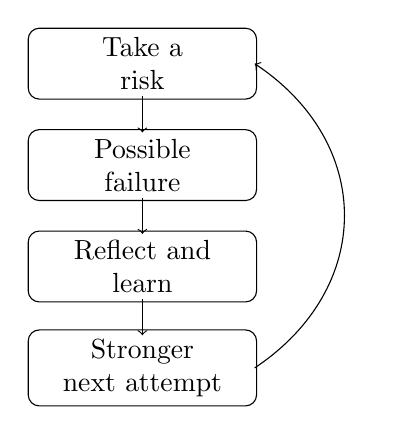
\begin{tikzpicture}[scale=0.92]
\node[draw, rounded corners, align=center, minimum width=2.9cm, minimum height=0.8cm] at (0,0) {Take a\\risk};
\node[draw, rounded corners, align=center, minimum width=2.9cm, minimum height=0.8cm] at (0,-1.4) {Possible\\failure};
\node[draw, rounded corners, align=center, minimum width=2.9cm, minimum height=0.8cm] at (0,-2.8) {Reflect and\\learn};
\node[draw, rounded corners, align=center, minimum width=2.9cm, minimum height=0.8cm] at (0,-4.2) {Stronger\\next attempt};
\draw[->] (0,-0.45) -- (0,-0.95);
\draw[->] (0,-1.85) -- (0,-2.35);
\draw[->] (0,-3.25) -- (0,-3.75);
\draw[->] (1.55,-4.2) .. controls (3.2,-3.1) and (3.2,-1.1) .. (1.55,0);
\end{tikzpicture}

\paragraph{Conceptual reconstruction.}
The transcript gives the verbal loop: risk, failure, response, learning, and renewed action.
\end{figure}

The comfort zone now has a specific meaning. It is not merely a mood. It is the region where the feedback loop is weak because the action is too protected to produce new information. The speaker says that entering discomfort forces growth: new skills, lifestyle changes, adaptation, and learning the details of unfamiliar situations.

\section{Passion Must Meet Monetization}

The second lesson shifts from whether to act to what to act on. The speaker says to follow passion, but he immediately qualifies the point: passion should be aligned with something that can be monetized. The examples are deliberately broad: music, coding, sports, content, services, and products.

The useful equation is not

\begin{equation}
\text{passion} \longrightarrow \text{business}.
\end{equation}

That is too vague. The lecture's actual mechanism is closer to

\begin{equation}
\text{passion}+\text{monetization path}
\longrightarrow
\text{commercial effort}.
\end{equation}

Here a monetization path may mean content, a service, a product, or another way of attaching a market to the work. The speaker's claim is that sustained effort is easier when the work matters personally. But he does not say that caring is enough. The care has to be shaped into something another person will watch, buy, hire, or support.

That gives us a practical definition.

\begin{definition}
A monetizable passion is an activity the person cares about, together with a concrete channel through which that activity can create value for others and receive payment, attention, or opportunity in return.
\end{definition}

The warning in the transcript is also important. The speaker contrasts long-term care with short-term gain. Work done only because it looks profitable can be hard to sustain. Work done only because it feels meaningful may never become a business. The entrepreneurial target is the intersection.

\begin{equation}
\text{entrepreneurial fit}
=
\text{personal energy}
\cap
\text{market demand}.
\end{equation}

This is a standard reconstruction of the transcript's point, not a literal equation from the video. It is useful because it keeps the two halves visible.

\section{Start Sooner, Before the Idea Becomes Delay}

The third lesson follows naturally. Once we have a passion and a possible monetization route, the next question is timing. The speaker gives a familiar sequence: a person says they will build a business, start a podcast, or open a store; then the start date becomes next month, six months, a year, and finally nothing.

The mathematical payload is opportunity cost. Delay is not neutral. Delay consumes time that could have produced feedback. If \(F(t)\) denotes accumulated market feedback by time \(t\), then a person who starts at time \(s\) has, very roughly,

\begin{equation}
F(t;s)=\int_s^t f(\tau)\,d\tau,
\end{equation}

where \(f(\tau)\) is the rate at which action produces feedback. If the start time \(s\) moves later, the interval of learning shrinks.

\begin{equation}
s_2>s_1
\quad\Longrightarrow\quad
F(t;s_2)\leq F(t;s_1)
\end{equation}

assuming the same feedback rate. This is not in the transcript as calculus, but it captures the speaker's practical claim: waiting reduces the number of chances to learn.

\subsection{Question \& Answer}

\paragraph{Question.}
What makes waiting costly if the idea is still there later?

\paragraph{Answer.}
The idea may still be there, but the learning has not happened. The speaker's concern is not simply calendar time. It is postponed contact with reality. We can write the update rule for an entrepreneurial project as

\begin{align}
I_{n+1} &= I_n + \text{feedback from attempt } n,\\
A_{n+1} &= A_n + \text{skill gained from attempt } n.
\end{align}

Here \(I_n\) is information about the market, and \(A_n\) is ability. If there is no attempt, both updates are weak. Starting sooner matters because the project begins to produce evidence.

This is also why the third lesson is tied to the second. Passion gives energy, but starting converts energy into observation. The speaker's phrase that starting sooner is critical should be read in this practical sense.

\section{Network as a Form of Leverage}

The fourth lesson expands the frame from individual effort to social structure. The speaker says to build a network, surround yourself with like-minded people, find mentors, and stay close to people who have done what you want to do. He also notes that entrepreneurship can become lonely, so the network is not only a source of information. It is also a support system.

There are several distinct objects inside the word network:

\begin{itemize}
\item mentors who have already scaled a business or reached the desired point;
\item peers with similar ambitions;
\item supporters who encourage the work;
\item critics who can correct the work constructively;
\item event contacts found through local communities, conventions, and industry gatherings.
\end{itemize}

The speaker then connects this back to the first lesson. His own platform had to reach out to multi-millionaires and business owners. Sometimes the ask was small: ten or fifteen minutes, lunch, or a brief conversation. The point is that outreach is a risk-bearing action. It may be uncomfortable, but it creates access.

A compact way to model the leverage is

\begin{equation}
\text{network value}
\approx
\text{access}
+
\text{information}
+
\text{accountability}.
\end{equation}

The transcript's quantitative detail is modest but concrete: even \(10\) or \(15\) minutes with the right person can carry value. We should not inflate that into a universal law. But it does show the shape of the advice: a small meeting can be worthwhile if it transfers specific context that would otherwise take much longer to learn.

\begin{figure}
\centering
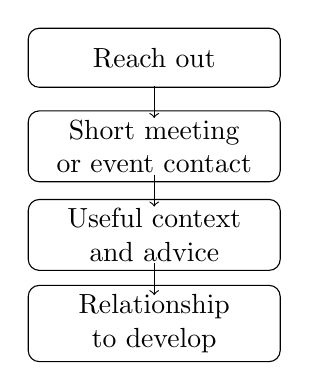
\begin{tikzpicture}[scale=0.9]
\node[draw, rounded corners, align=center, minimum width=3.2cm, minimum height=0.75cm] at (0,0) {Reach out};
\node[draw, rounded corners, align=center, minimum width=3.2cm, minimum height=0.75cm] at (0,-1.25) {Short meeting\\or event contact};
\node[draw, rounded corners, align=center, minimum width=3.2cm, minimum height=0.75cm] at (0,-2.5) {Useful context\\and advice};
\node[draw, rounded corners, align=center, minimum width=3.2cm, minimum height=0.75cm] at (0,-3.75) {Relationship\\to develop};
\draw[->] (0,-0.4) -- (0,-0.85);
\draw[->] (0,-1.65) -- (0,-2.1);
\draw[->] (0,-2.9) -- (0,-3.35);
\end{tikzpicture}

\paragraph{Conceptual reconstruction.}
The networking lesson moves from outreach to small contact, then to information, then to relationship-building.
\end{figure}

The rhythm of the lecture matters here. The speaker does not jump directly from ``network'' to ``go to events.'' He first talks about mentors, then support, then criticism, then outreach, then local conventions. A faithful chapter should preserve that widening motion: inner circle, experienced guides, active outreach, public events.

\section{Let Money Work Through Assets}

The final lesson is capital allocation. The speaker says that multi-millionaires did not merely let money sit in the bank or spend all of it. They took money earned from careers or businesses and put it into tangible assets such as real estate, or into stocks. He also mentions that many people now invest in cryptocurrency. The common mechanism is that money is being placed where it may grow.

The caution is essential. The lecture's examples are not guarantees. They are categories named by the speaker. The defensible claim is comparative:

\begin{equation}
\text{idle cash} \quad \hbox{versus} \quad \text{assets with possible appreciation}.
\end{equation}

If \(\pi\) denotes inflation and \(y_{\text{bank}}\) denotes the yield on bank deposits, then the purchasing power of idle cash is pressured whenever

\begin{equation}
\pi > y_{\text{bank}}.
\end{equation}

In that case, the real value of the bank balance declines even if the nominal number of dollars is unchanged. This is the standard financial form of the speaker's statement that money sitting in a bank goes down in value over time with inflation.

For an appreciating asset, a simple model is

\begin{equation}
V_t=V_0(1+r)^t,
\end{equation}

where \(V_0\) is the initial value, \(V_t\) is the later value, and \(r\) is the rate of appreciation. This equation should be read cautiously. The transcript does not promise \(r>0\). It says that multi-millionaires often try to put money into places where appreciation is possible.

\paragraph{Worked example.}
Suppose idle cash earns \(y_{\text{bank}}=1\%\) while inflation is \(\pi=4\%\). The approximate annual change in purchasing power is

\begin{equation}
y_{\text{bank}}-\pi = 1\%-4\%=-3\%.
\end{equation}

So the money may look stable in nominal terms while losing real purchasing power. Now suppose an asset grows at \(r=5\%\) for three years. The simple compounding model gives

\begin{align}
V_3 &= V_0(1.05)^3\\
    &\approx 1.158V_0.
\end{align}

The example does not recommend any particular asset. It only illustrates the distinction the speaker is making: idle money and allocated money have different dynamics.

\begin{figure}
\centering
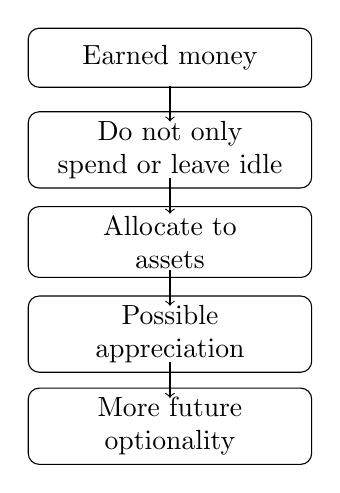
\begin{tikzpicture}[scale=0.9]
\node[draw, rounded corners, align=center, minimum width=3.6cm, minimum height=0.75cm] at (0,0) {Earned money};
\node[draw, rounded corners, align=center, minimum width=3.6cm, minimum height=0.75cm] at (0,-1.3) {Do not only\\spend or leave idle};
\node[draw, rounded corners, align=center, minimum width=3.6cm, minimum height=0.75cm] at (0,-2.6) {Allocate to\\assets};
\node[draw, rounded corners, align=center, minimum width=3.6cm, minimum height=0.75cm] at (0,-3.9) {Possible\\appreciation};
\node[draw, rounded corners, align=center, minimum width=3.6cm, minimum height=0.75cm] at (0,-5.2) {More future\\optionality};
\draw[->] (0,-0.4) -- (0,-0.9);
\draw[->] (0,-1.7) -- (0,-2.2);
\draw[->] (0,-3.0) -- (0,-3.5);
\draw[->] (0,-4.3) -- (0,-4.8);
\end{tikzpicture}

\paragraph{Conceptual reconstruction.}
The asset lesson converts earned money into a sequence: avoid idle use, allocate, allow possible appreciation, and create future optionality.
\end{figure}

This final lesson also completes the lecture's arc. The earlier sections are about producing action and access. The last section asks what happens after money is earned. The speaker's answer is ownership of assets rather than passive holding or consumption.

\section{Summary}

The five lessons form one chain. We begin with risk because action is required before learning can occur. We then ask what the action should be attached to, and the answer is passion joined to a monetization path. We then ask when to begin, and the answer is sooner, because delay reduces feedback cycles.

The fourth lesson adds other people to the model: mentors, peers, supporters, critics, short meetings, and local events. The fifth lesson adds capital allocation: earned money should not merely sit idle or be spent, but may be placed into assets where appreciation is possible. The chapter's compact structure is therefore

\begin{equation}
\text{risk}
\longrightarrow
\text{monetized passion}
\longrightarrow
\text{early action}
\longrightarrow
\text{network leverage}
\longrightarrow
\text{asset ownership}.
\end{equation}

That is the lecture's business logic. It is interview-derived, practical, and not a guarantee. But it is coherent: act, learn, align the work, start before the idea decays, build access to people, and convert earnings into assets that can work over time.